\thispagestyle{fancy}
\begin{center}
	\LARGE{\textbf{Ley de ohm (Segunda parte)}}
\end{center}
\section{Objetivos}
Al finalizar esta experiencia, usted estará capacitado para:
\begin{enumerate}
	\item Calcular la conductancia en circuitos paralelos.
	\item Calcular la corriente usando el principio de los divisores.
	\item Medir la corriente en circuitos paralelos y comprobar el principio de los divisores de corriente.
\end{enumerate}
\section{Conocimientos previos}
Un divisor de corriente es una red de resistores en paralelo que se repartan entre ellos la corriente.
\begin{equation*}
	\centering
	I = \frac{ Conductancia seleccionada }{ conducatancia total en paralelo}I_{Total}
\end{equation*}
\textbf{Donde:}
\\ Conductancia $= G = \frac{1}{R}$
\section{Autoevaluación de entrada}
Estudie el circuito de la siguiente figura 1 y  conteste las preguntas.
\begin{figure}[h]
	\centering
	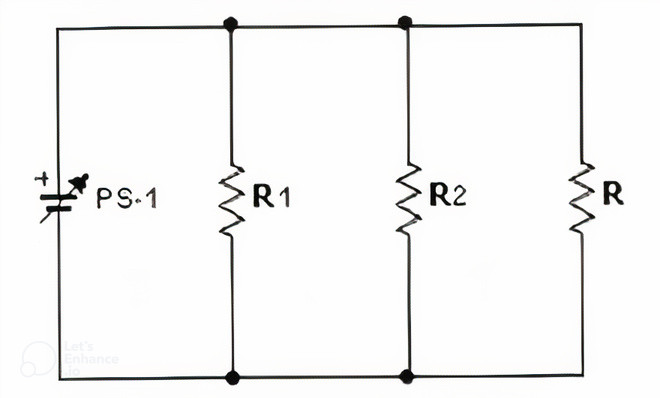
\includegraphics[scale=0.5]{imagenes/1}
	\caption{Circuito ha armarse}
\end{figure}
\begin{enumerate}
	\item En la figura 1 si $R_{1} =10\Omega$ y $V=10V$. ¿Cuánta corriente fluye por $R_{1}$?\\ $ V=IR_{1}
	10=I*10→I=1A , I=1A$
	
	\item En la figura 1 si $R_{2} =40\Omega$ y $V=6V$. ¿Cuánta corriente fluye por $R_{2}$?\\ $V=IR_{2}
	6=I*40, I=0.15A, I=0.15A$
	
\end{enumerate}
\section{Equipo}
El siguiente equipo es necesario para realizar el experimento.
\begin{enumerate}
	\item Módulo de experimentos.
	\item DMM (Multímetro digital).
\end{enumerate}
\section{Procedimiento}
\begin{enumerate}
	\item Conecte el circuito que contiene los resistores $R_{1}$, $R_{2}$ y $R_{3}$, como se muestra en la siguiente figura. 
	\begin{figure}[h]
		\centering 
		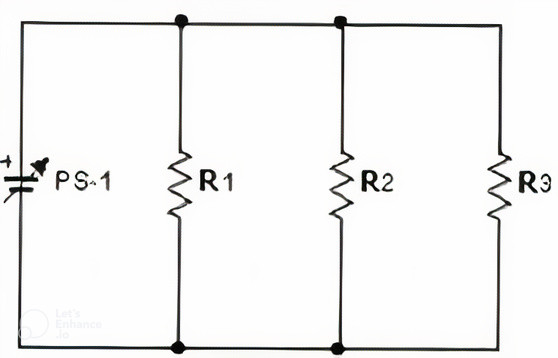
\includegraphics[scale=0.5]{imagenes/5}
		\caption{Segundo circuito a armarse}
	\end{figure}
	\item Lleve la salida de las fuentes de alimentación de 0 V. Conecte el divisor de corriente.
	\item Fije la salida PS-1 en 10 V.
	\item Calcule y anote las conductancias de $R_{1}$, $R_{2}$ y$ R_{3}$ (tome tres digitos después de la coma).
	\\ La unidad de conductancia es el Siemens (a veces llamado mho). La  conductancia de un resistor de $2k\Omega$ en 0.5 mS.
\begin{table}[h]
	\centering
	
	\begin{tabular}{|c|c|}
		\hline
		$G_{1}$&0.5mA\\ \hline 
		$G_{2}$&0.37mA\\ \hline
		$G_{3}$&0.33mA\\ \hline
		$G_{eq}$=$G_{1}$ + $G_{2}$+$G_{3}$&1.208mA\\ \hline
		
	\end{tabular}
	\caption{}
\end{table}
\item Mida la corriente entrante al divisor de corriente:\\
$I_{salida}=4.5mA$
	\item Usando la ecuación:
	\begin{equation*}
		I_{sal} = \frac{Conductancia seleccionada}{Conductancia total en paalelo}I_{ent}
	\end{equation*}
	\\ Calcule y registre la corriente de salida 
	
	\begin{table}[h]
		\centering
		\begin{tabular}{|c|c|}
			\hline
			$I_{sal}$ en &$R_{1}$ = 1.5mA\\ \hline
			&$R_{2}=1.5mA$\\ \hline
			&$R_{3}= 1.5mA$\\ \hline			
		\end{tabular}
		\caption{}
	\end{table}
	\item Compruebe los cálculos midiendo la corriente en los tres resistores. Registre sus resultados en el siguiente cuadro:
	\begin{table}[h]
		\centering
		\begin{tabular}{|c|c|}
			\hline
			$I_{sal}$ en &$R_{1}$ = 1.5mA\\ \hline
			&$R_{2}=1.5mA$\\ \hline
			&$R_{3}= 1.5mA$\\ \hline			
		\end{tabular}
		\caption{}
	\end{table}
	\\ Comparte los valores medidos con los calculados.
\end{enumerate}
\section{Autoevaluación}
\begin{enumerate}
	\item Por tres resistores $10\Omega, 27\Omega$ y $56\Omega$ conectadas en paralelo circula una corriente de 1A. ¿Cuál es la corriente que circula por el resistor de $10\Omega$?
	\begin{figure}[h]
		\centering
		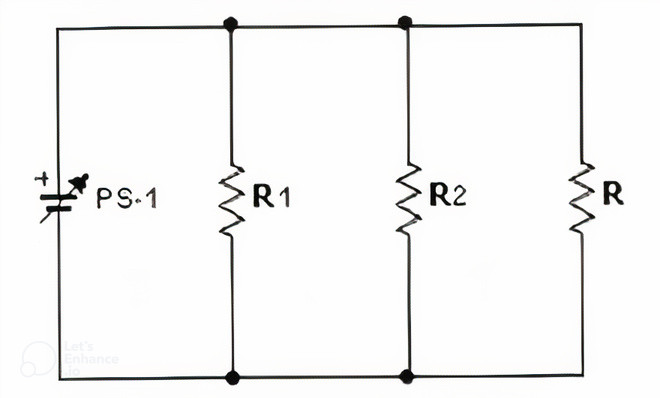
\includegraphics[scale=1]{imagenes/1}
	\end{figure}
	\\ Solución: 
	\begin{equation*}
		0I_{1}=27I_{2}=56I_{3}=k, I_{1}=\frac{k}{10}, I_{2}=\frac{k}{27}, I_{3}=\frac{k}{56}
	\end{equation*}
	\begin{equation*}
		I_{1}+ I_{2}+I_{3}=1,  \frac{k}{10}+\frac{k}{27}+\frac{k}{56}, k=6.4560, I_{1}= 0.6456mA
	\end{equation*}
	\item Por tres resistores $10\Omega, 27\Omega$ y $56\Omega$ conectadas en paralelo circula una corriente de 1A. ¿Cuál es la corriente que circula por el resistor de $27\Omega$?
	\begin{figure}[h]
		\centering
		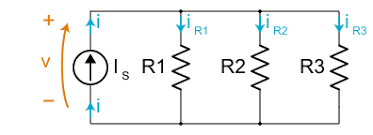
\includegraphics[scale=1]{imagenes/2}
	\end{figure}
	\begin{equation*}
		V=10I_{1}, V=27I_2{}, V=56I_{3}
	\end{equation*}
	\\
	Solución:
	\begin{equation*}
		0I_{1}=27I_{2}=56I_{3}=k, I_{1}=\frac{k}{10}, I_{2}=\frac{k}{27}, I_{3}=\frac{k}{56}
	\end{equation*}
	\begin{equation*}
		I_{1}+ I_{2}+I_{3}=1,  \frac{k}{10}+\frac{k}{27}+\frac{k}{56}, k=6.4560, I_{2}= 0.2391mA
	\end{equation*}
	\item Por tres resistores $10\Omega, 27\Omega$ y $56\Omega$ conectadas en paralelo circula una corriente de 1A. ¿Cuál es la corriente que circula por el resistor de $56\Omega$?
	\begin{figure}[h]
		\centering
		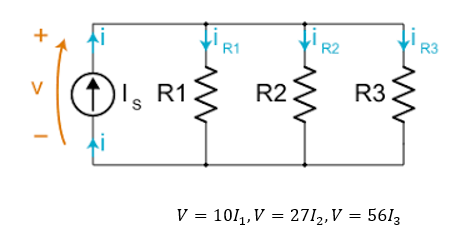
\includegraphics[scale=1]{imagenes/3}
	\end{figure}
	\\Solución:
	\begin{equation*}
		10I_{1}=27I_{2}=56I_{3}=k I_{1}=\frac{K}{10},I_{2}=\frac{k}{27},I_{3}=\frac{k}{56}
	\end{equation*}
	\begin{equation*}
		I_{1}+ I_{2}+I_{3}=1
	\end{equation*}
	\begin{equation*}
		\frac{k}{10}+\frac{k}{27}+\frac{k}{56}=1, k=6.4560  
	\end{equation*}
	\begin{equation*}
		I_{3}=\frac{6.4560}{56}=0.1153 A
	\end{equation*}
\end{enumerate}
\section{Conclusión}
Las fórmulas para cada caso son de suma importantes ya que nos ayudan a resolver los circuitos eléctricos también llevar a cabo en la simulación es bueno ya que así veremos los cambios que se puedan suscitar.

